
\فصل{مطالب تکمیلی}
\قسمت{ابرپارامتر‌های مدل‌ها}
برای تست و بررسی مدل‌ها از کتابخانه \lr{scikit survival} و \lr{pycox} استفاده شد. این کتابخانه‌ها مبتنی بر مقالات موجود، به پیاده‌سازی مدل‌های ارائه شده پرداخته‌اند و تست و بررسی آن‌ها روی داده‌ها به کمک این کتاب‌خانه‌ها ساده‌تر است.

در خصوص ابرپارامترها، برای هر یک از مدل‌ها از مجموعه‌ی ابرپارامترهای زیر استفاده شد. برای یافتن بهترین ابرپارامترها، از جستجوی همگانی و \lr{Grid Search} استفاده گردید.

\شروع{فقرات}
\فقره مدل جنگل بقا 
(
\texttt{sksurv.ensemble.RandomSurvivalForest}):
\begin{latin}
\footnotesize
\begin{verbatim}
max_features: 'sqrt', min_samples_leaf: 3, min_samples_split: 3, n_estimators: 50
\end{verbatim}\end{latin}
\فقره
مدل تقویت گرادیان 
(
\texttt{sksurv.ensemble.GradientBoostingSurvivalAnalysis}
):
\begin{latin}
\footnotesize
\begin{verbatim}
learning_rate: 0.05, loss: 'coxph', min_samples_leaf: 8, min_samples_split: 2, n_estimators: 1000
\end{verbatim}\end{latin}
\فقره
مدل \lr{Cox-PH}
( 
\texttt{sksurv.linear\_model.CoxPHSurvivalAnalysis}
):
\begin{latin}
\footnotesize
\begin{verbatim}
alpha: 0, n_iter: 50, ties: 'efron', tol: 1e-09
\end{verbatim}\end{latin}
\فقره
مدل \lr{Deep Surv}
(
\texttt{pycox.models.CoxPH}
):
\begin{latin}
\footnotesize
\begin{verbatim}
network structure: [64, 64, 64]
batch_norm: True
dropout: 0.6
initial_lr: 0.01
\end{verbatim}
\end{latin}
\فقره
مدل \lr{Logistic Hazard}
(
\texttt{pycox.models.LogisticHazard}
):
\begin{latin}
	\footnotesize
	\begin{verbatim}
	num_nodes: [64, 128, 128, 64]
	batch_norm: True
	dropout: 0.65
	initial_lr: 0.05
	optimizer: AdamWR
	\end{verbatim}
\end{latin}
\فقره
مدل \lr{PC Hazard}
(
\texttt{pycox.models.PCHazard}
):
\begin{latin}
	\footnotesize
	\begin{verbatim}
	num_nodes: [16, 32, 16]
	batch_norm: True
	dropout: 0.8
	initial_lr: 0.05
	optimizer: Adam
	\end{verbatim}
\end{latin}
\پایان{فقرات}

\قسمت{توزیع $C_{index}$ در آزمایش‌های جستجوی کامل و نیمه‌کامل}
در شکل~\رجوع{شکل:توزیع‌جستجو‌ها} می‌توان توزیع معیار $C_{index}$ را در آزمایشات مربوط به انتخاب ویژگی‌ها مشاهده کرد. همانطور که مشاهده می‌شود، مقدار $C_{index}$ در محدوده‌ی 
$\left[0.7, 0.9\right]$
می‌ماند که با توجه به نتایج آزمایش‌هایمان، بازه‌ای قابل قبول است. ضمنا همین توزیع‌ها نشان می‌دهند که می‌توان تعدادی زیادی از ویژگی‌ها را حذف کرد و همچنان دقتی در حد دقت گزارش شده در فصل‌های پیشین که با در نظر گرفتن همه‌ی ویژگی‌ها بود داشت. این موضوع نشان می‌دهد که تعدادی از ویژگی‌های ما عملاً دانش زیادی اضافه نمی‌کنند و نبودنشان اثری ندارد.

در آزمایش جستجوی کامل، حد پایین $0.83$ برای انتخاب مجموعه‌‌های امیدبخش در نظر گرفته شده است. اما در آزمایش جستجوی‌ نیمه‌کامل حد $0.835$ در نظر گرفته شده است. احتمال موجود در تصاویر برای هر ویژگی، با تقسیم تعداد مجموعه‌هایی امیدبخشی که ویژگی مربوطه را دارند بر تعداد کل مجموعه‌های امیدبخش به دست آمده است.

\pgfplotsset{width=7.5cm,compat=1.12}
\usepgfplotslibrary{fillbetween}
\شروع{شکل}
[t]\centering
\begin{latin}
	\hspace*{-0.04\linewidth}
	\footnotesize
	\begin{subfigure}[t]{0.45\textwidth}
	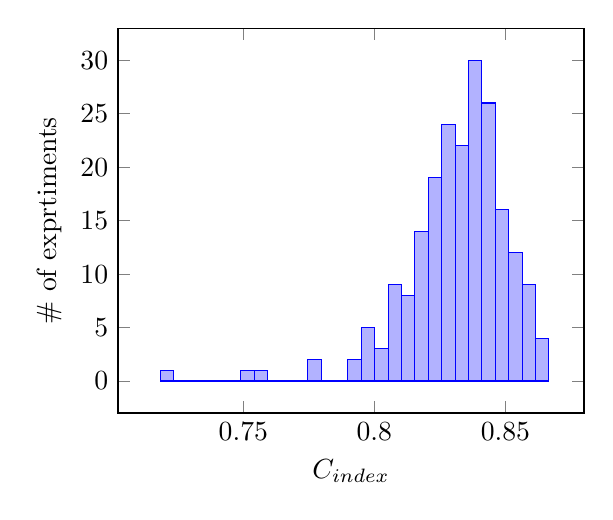
\begin{tikzpicture}
	\begin{axis}[
	area style,
	xtick={0.70, 0.75, ..., 0.85},
	ytick={0, 5, ..., 40},
	xmax=0.88,
	ylabel=\# of exprtiments,
	xlabel=$C_{index}$
	]
	\addplot+[ybar interval,mark=no] plot coordinates {
		(0.7183191, 1.0)
		(0.723433, 0.0)
		(0.7285468, 0.0)
		(0.7336607, 0.0)
		(0.7387746, 0.0)
		(0.7438885, 0.0)
		(0.7490023, 1.0)
		(0.7541162, 1.0)
		(0.7592301, 0.0)
		(0.764344, 0.0)
		(0.7694578, 0.0)
		(0.7745717, 2.0)
		(0.7796856, 0.0)
		(0.7847995, 0.0)
		(0.7899134, 2.0)
		(0.7950272, 5.0)
		(0.8001411, 3.0)
		(0.805255, 9.0)
		(0.8103689, 8.0)
		(0.8154827, 14.0)
		(0.8205966, 19.0)
		(0.8257105, 24.0)
		(0.8308244, 22.0)
		(0.8359382, 30.0)
		(0.8410521, 26.0)
		(0.846166, 16.0)
		(0.8512799, 12.0)
		(0.8563937, 9.0)
		(0.8615076, 4.0)
		(0.8666215, 2.0)
	};
	\end{axis}
	\end{tikzpicture}
	\caption{Exhaustive Search}
	\end{subfigure}
	\hfill
	\begin{subfigure}[t]{0.45\textwidth}
	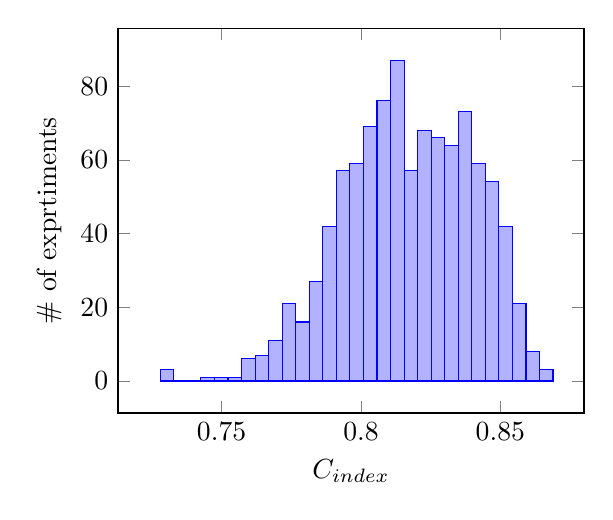
\begin{tikzpicture}
	\begin{axis}[
	area style,
	xtick={0.70, 0.75, ..., 0.85},
	ytick={0, 20, ..., 160},
	xmax=0.88,
	ylabel=\# of exprtiments,
	xlabel=$C_{index}$
	]
	\addplot+[ybar interval,mark=no] plot coordinates {
		(0.7280231, 3.0)
		(0.7328811, 0.0)
		(0.737739, 0.0)
		(0.742597, 1.0)
		(0.747455, 1.0)
		(0.752313, 1.0)
		(0.757171, 6.0)
		(0.762029, 7.0)
		(0.7668869, 11.0)
		(0.7717449, 21.0)
		(0.7766029, 16.0)
		(0.7814609, 27.0)
		(0.7863189, 42.0)
		(0.7911768, 57.0)
		(0.7960348, 59.0)
		(0.8008928, 69.0)
		(0.8057508, 76.0)
		(0.8106088, 87.0)
		(0.8154668, 57.0)
		(0.8203247, 68.0)
		(0.8251827, 66.0)
		(0.8300407, 64.0)
		(0.8348987, 73.0)
		(0.8397567, 59.0)
		(0.8446147, 54.0)
		(0.8494726, 42.0)
		(0.8543306, 21.0)
		(0.8591886, 8.0)
		(0.8640466, 3.0)
		(0.8689046, 1.0)
	};
	\end{axis}
	\end{tikzpicture}
	\caption{Semi-Exhaustive Search}
	\end{subfigure}
\end{latin}
\شرح{توزیع $C_{index}$ در مجموعه آزمایشات جستجوی کامل و جستجوی نیمه‌کامل. شکل سمت چپ مربوط به $210$ آزمایش  جستجوی کامل؛ هنگامی که مدل \lr{Logistic Hazard} روی مجموعه‌ی $19$ عضوی از ویژگی‌ها آموزش ببیند. شکل سمت راست مربوط به $1000$ آزمایش جستجوی نیمه‌کامل؛ هنگامی که مدل \lr{Logistic Hazard} روی مجموعه‌ی $15$ عضوی از ویژگی‌ها آموزش می‌بیند. }
\برچسب{شکل:توزیع‌جستجو‌ها}
\پایان{شکل}

